\documentclass{article}
\usepackage{amsmath}
\usepackage{amssymb}
\usepackage{amsfonts}
\usepackage{dsfont}
\usepackage{graphicx} % Required for inserting images
\usepackage{listings}
	\lstset{language=R,
    basicstyle=\small\ttfamily,
    stringstyle=\color{green},
    otherkeywords={0,1,2,3,4,5,6,7,8,9},
    morekeywords={TRUE,FALSE},
    deletekeywords={data,frame,length,as,character},
    keywordstyle=\color{blue},
    commentstyle=\color{green},
}
\usepackage{xcolor}
\usepackage{array}
\usepackage[vmargin=2cm,hmargin=2cm]{geometry}


\title{TP4 - Analyse des correspondances multiples}
\author{Guillaume Bernard-Reymond et Lorenzo Gaggini}
\date{Janvier 2024}

\begin{document}
\newcommand{\norme}[1]{\left\| #1\right\|}
\newcommand{\tr}{\text{tr}}
\maketitle
\setlength{\parindent}{0pt}

Dans ce TP, nous avons à notre disposition un jeu données concernant 300 consommateurs de thé ayant répondu à un questionnaire de 36 questions dont les réponses sont qualitatives, hormis une concernant l'âge. 

Nous avons décidé d'utiliser la bibliothèque FactomineR pour son confort d'utilisation. On trouvera le code R utilisé en appendice.

\begin{enumerate}
\item \textbf{L'ACM}

	\begin{enumerate}
	\item \textbf{Description des commandes }
	
	Les 18 premières variables correspondent aux modes de consommation du thé, la 19-ème est l'âge des personnes. Enfin les 17 dernières variables nous informent sur la personne et sa perception du thé. On met donc en relation le mode consommation avec l'individu et sa perception du thé. C'est ce qui justifie la mise en supplémentaire de ces 17 variables.
	
	\item Les deux premières dimensions captent 17,988\% de la part de variance totale comme l'illustre le tableau ci-dessous : 
	
\begin{center}
\begin{tabular}{|c|c|c|c|c|c|c|c|}
\hline 
& Dim.1 &  Dim.2 &  Dim.3 &  Dim.4 &  Dim.5 &  Dim.6  & Dim.7 \\ 
\hline 
Variance & 0.148 &  0.122 &  0.090 &  0.078 &  0.074  & 0.071 &  0.068\\ 
\hline 
\% of var.   & 9.885 &  8.103 &  6.001 &  5.204 &  4.917 &  4.759 &  4.522\\ 
\hline 
Cumulative \% of var.  & 9.885 & 17.988 & 23.989 & 29.192  & 34.109 & 38.868 & 43.390 \\ 
\hline 
\end{tabular} 
\end{center}
	                      
De plus sur le graphique des valeurs propres, on peut observer un décrochement après la deuxième : 

\begin{center} 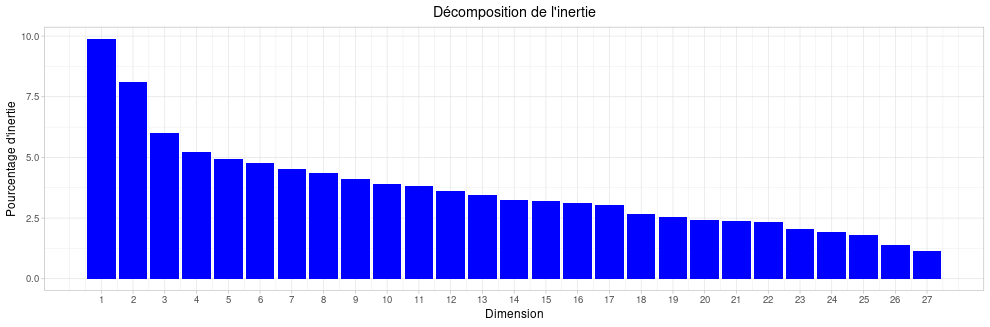
\includegraphics[width=\linewidth]{image/vp.png}\end{center}	                      
	
	Tableau des individus les plus contributeurs pour l'axe 1 : 
	
	\begin{center}
\begin{tabular}{|c|c|c|c||c|c|c|c|}
\multicolumn{4}{c}{Côté -} & \multicolumn{4}{c}{Côté +}\\
\hline 
Individus & Coordonnées & CTR & COS2 & COS2 & CTR & Coordonnées & Individus \\ 
\hline 
262 & $-0.71$ & $5.55$ & $0.51$ & $0.75$ & $8.19$ & $0.86$ & 265  \\ 
\hline 
205 &  &  &  & $0.71$ & $7.85$ & $0.85$ & 273\\  
\hline 
\end{tabular} 
\end{center}

\begin{center}
\begin{tabular}{cc}
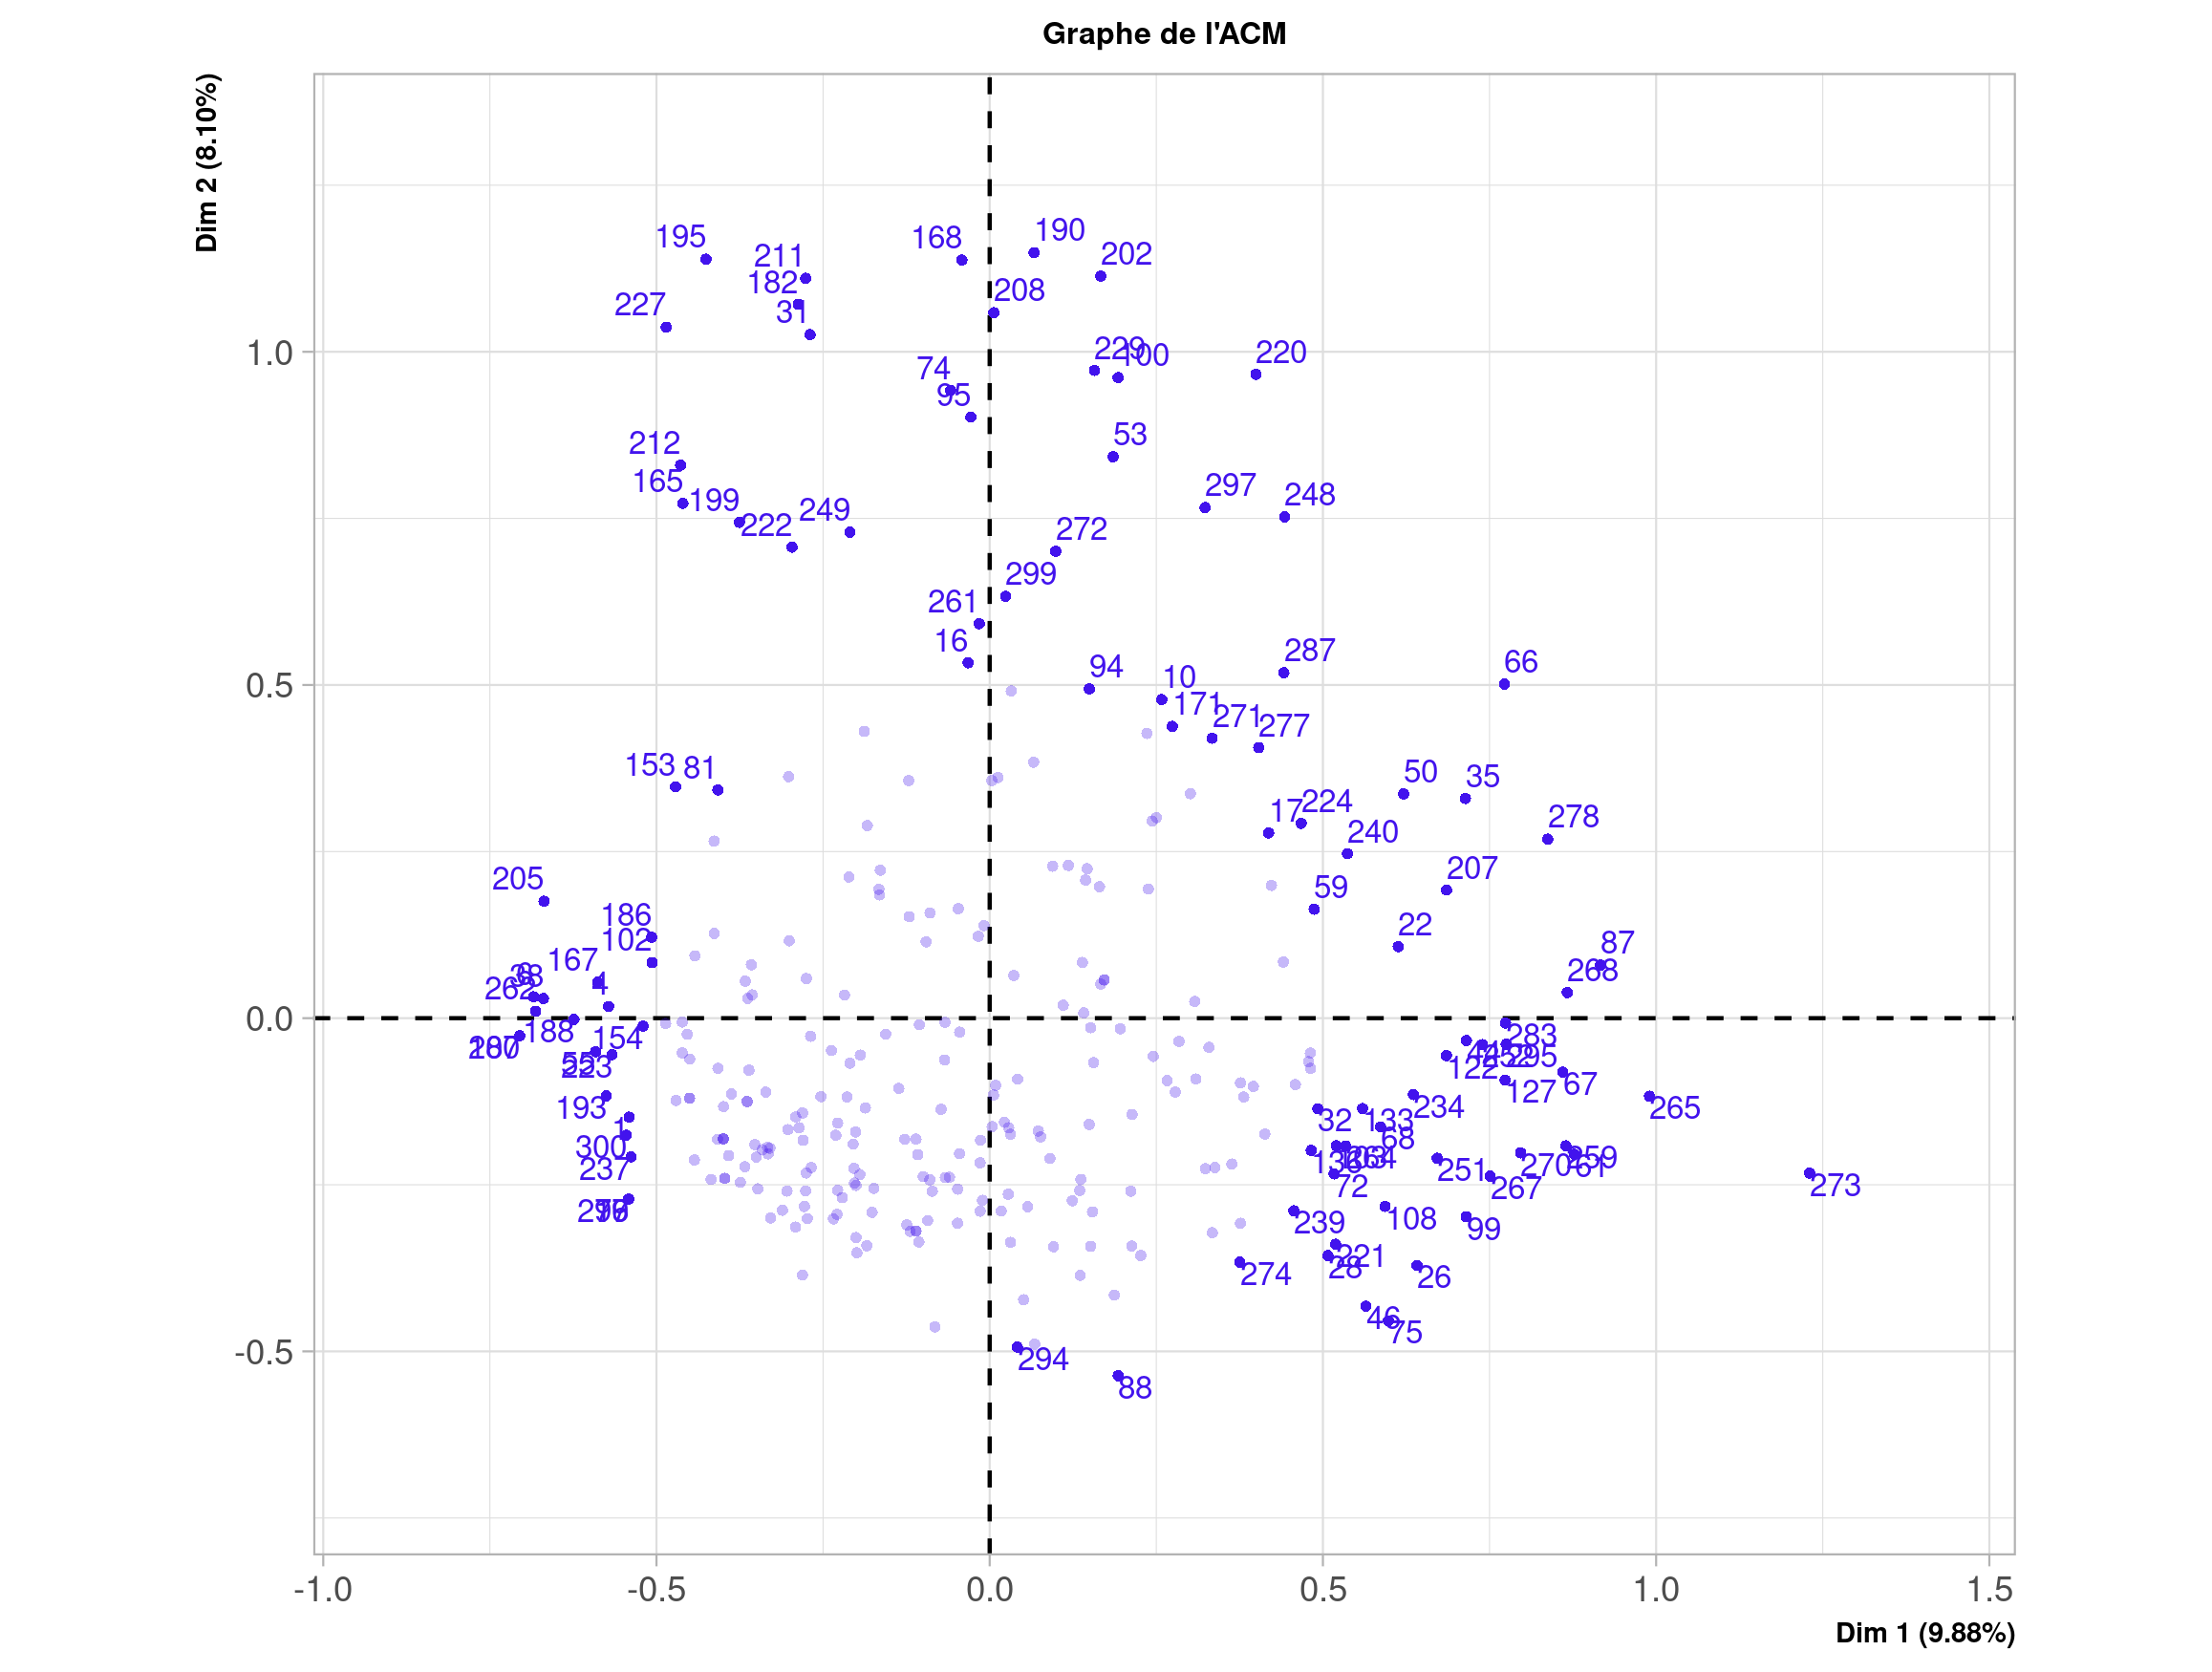
\includegraphics[width=0.48\linewidth]{image/indiv_100} &  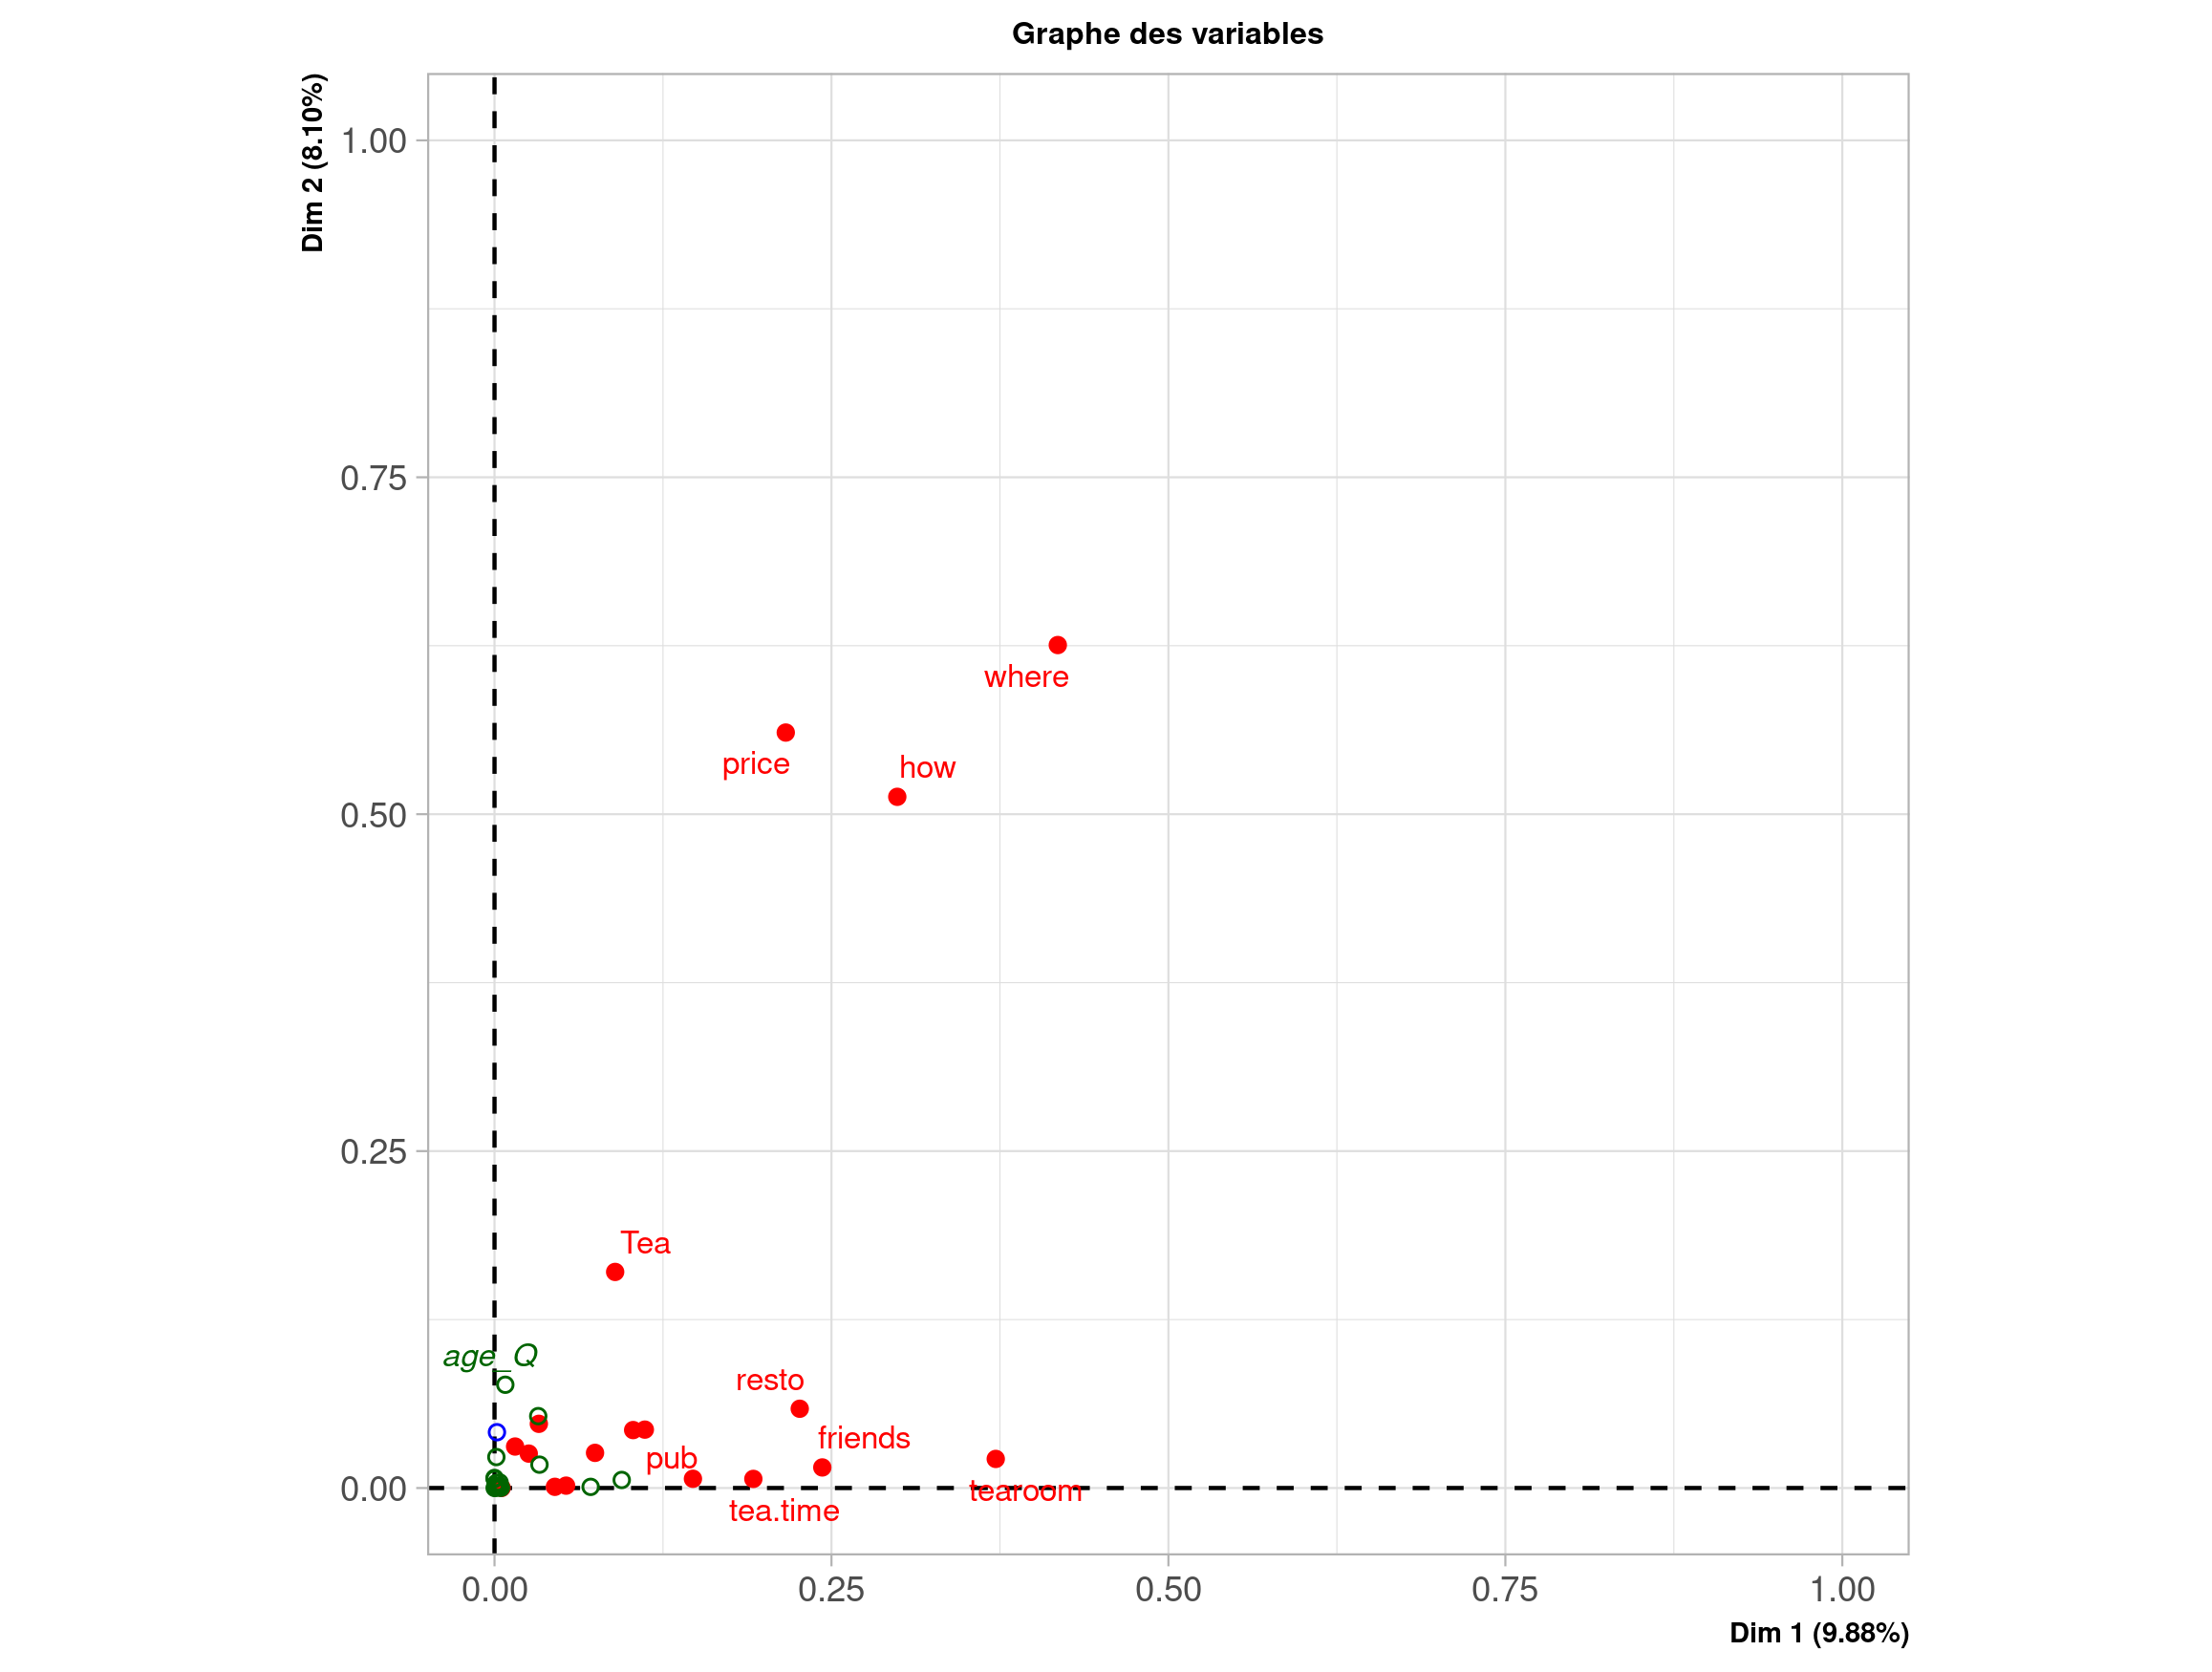
\includegraphics[width=0.48\linewidth]{image/variables} \\
Graphe des 100 individus les plus contributeurs & Graphe des variables 
\end{tabular} 
\end{center}



Pour ce qui est des variables, les plus liées à la première dimension sont : "where" ($R^2=0.418$); "tearoom" ($R^2=0.372$) et "how" ($R^2=0,299$)


\textbf{Dimension 2}

Sur le second, on peut voir s'opposer des individus (168; 190)  en haut et (88; 294) en bas. Toutefois, on ne distingue pas d'individus particulier qui aurait contribué de façon majeure au positionnement de cette axe.

Du côté des variables, on retrouve deux des trois variables précédentes : "where" ($R^2=0.626$), "price" ($R^2= 0.561$) et "how" ($R^2=0.513$).
	\end{enumerate}
	
\item \textbf{Etude des individus}
	\begin{enumerate}
	\item Aucun groupe ne se dégage de manière suffisamment significative pour être interprété. Le nuage est étalé de manière homogène.
	\item Les individus atypiques sont ceux remarqués à la question 1)b) à savoir les individus 273 et 265. Ce sont des consommateurs buvant du thé de manière régulière sans contexte particulier. L'individu 205 illustre en opposition sur cet axe le mode de consommation.\\
	
On voit sur le tableau suivant l'opposition des individus 273 et 205.
	
\begin{center}
\begin{tabular}{|c|c|}
\hline
Individu 273 &  Individu 205 \\
\hline
breakfast & Not.breakfast\\
\hline
tea time & Not.tea time\\
\hline
evening & Not.evening\\
\hline
Not.lunch & Not.lunch\\
\hline
Not.dinner & dinner\\
\hline
always & Not.always\\
\hline
home & home\\
\hline
work & Not.work\\
\hline
tearoom & Not.tearoom\\
\hline
friends & friends \\
\hline
resto & Not.resto \\
\hline
pub & Not.pub \\
\hline
Earl Grey & green \\
\hline
other & alone \\
\hline
sugar & No.sugar \\
\hline
tea bag+unpackaged & tea bag \\
\hline
chain store+tea shop & chain store \\
\hline
p\_variable & p\_branded\\
\hline
\end{tabular}

\end{center}

	\end{enumerate}

\item \textbf{Etude des variables et des modalités :}

	\begin{enumerate}
	\item Les modalités opposées le long du premier axes sont : "tea room, chain store tea-shop" à "not friends, not tearoom, not tea-time". Cela appuie les oppositions relevées par les individus atypiques relevés précédemment entre les buveurs de thé réguliers et ceux ne l'étant pas.
	\item La seconde dimension oppose "teashop, unpackaged, p-upscale" à "p-unknow". C'est donc un mode de consommation propre à des amateurs avertis de thé.  
	\item Le graphique ci-dessous montre que l'âge n'est pas bien représenté le long de la dimension 2. Sa corrélation est seulement de 0,2.

\begin{center}
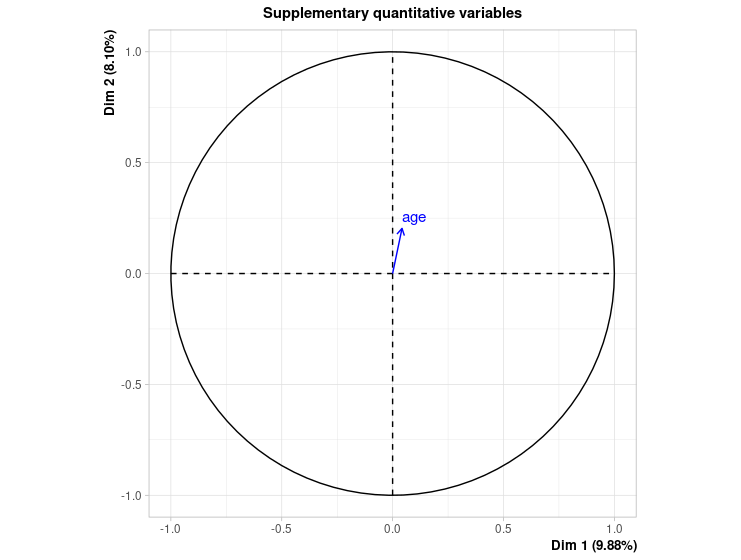
\includegraphics[width=0.7\linewidth]{image/age.png}
\end{center}
	
	 On comprend alors l'opposition entre les jeunes consommateurs et les plus âgés. Les premiers achètent du thé sans nécessairement se soucier de la qualité du thé consommé. A la différence des personnes plus âgées qui ont tendance à s'orienter vers des magasins spécialisés vendant du thé haut de gamme.
	\item Voici le graphique des modalités illustratives :
	
	\begin{center}
	 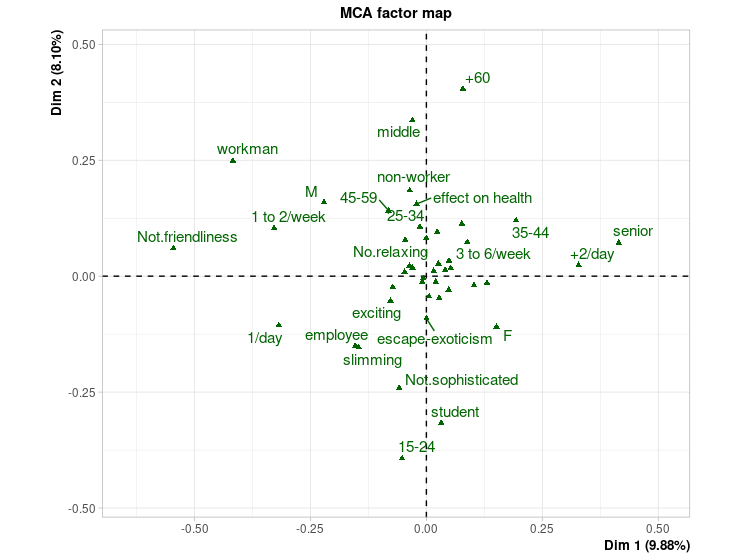
\includegraphics[width=0.6\linewidth]{image/modalite.png}
	 \end{center} 
	
	On peut observer que les modalités de la variable age-Q sont ordonnées de bas en haut, des plus jeunes aux plus âgés. Ceci corrobore l'orientation de la variable "âge" le long de l'axe 2. "Age-Q" et "age" étant deux représentations différentes d'une même quantité intrinsèque aux individus, elles sont en toute cohérence semblables.
	\end{enumerate}

\item \textbf{Ellipse de confiance}

qu'est ce que l'on  doit faire ???????
\end{enumerate}

\end{document}